\section{Cockroft Walton}\label{ch:cock}
\todo[color=c04x,inline]{testing the colors}
The Cockroft-Walton Boost Converter (CWBC) utilises passive components to multiply the output voltage of a CBC.
To achieve this the CWBC employs a Cockroft-Walton Half-Wave Multiplicator (CWHWM) instead of the output capacitor.
A general schematic of the CWHWM can be seen in Figure \ref{fig:CWHWM}.

\subsection{Additions from Conventional BC}
\begin{figure}[H]
   \centering
   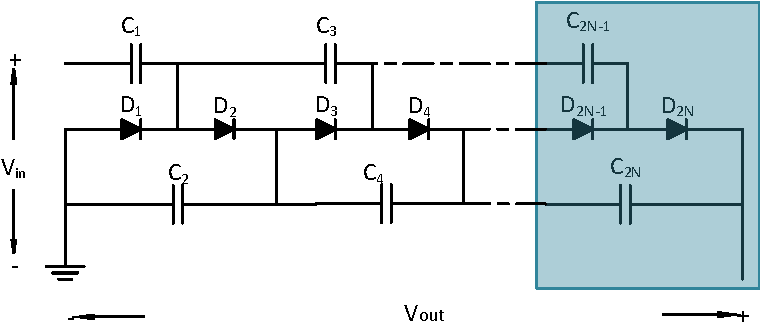
\includegraphics[width=0.6\textwidth]{figures/xCockroftWalton/CockroftWalton.pdf}
    \caption{Detailed view of the Cockroft-Walton Output capacitor substitution}
	\label{fig:CWHWM}
\end{figure}

The figure shows a three stage CWHWM,
with the third stage marked with a blue box.
Since all stages are equal and just appended to the previous,
more stages can be added at the dotted lines.

